\documentclass[portrait]{seminar}
%\usepackage{pandora}
\usepackage{color}
\usepackage{fancybox}
\usepackage{alltt}
\usepackage{epsfig}
\usepackage{rail}
\usepackage{bar}
\usepackage{url}
\usepackage{rotating}
\usepackage[normalem]{ulem}
\usepackage{latexsym}
\usepackage{amsmath}

\begin{document}

\boldmath
\newcommand{\RA}{$\rightarrow$}
\newcommand{\LL}{\mbox{$[$\hspace{-0.15em}$[$}}
\newcommand{\RR}{\mbox{$]$\hspace{-0.15em}$]$}}
\newcommand{\CC}[1]{\mbox{\tt $\LL$#1$\RR$}}

\slideframe{shadow}

%%% Activate one of these to get either Aarhus style or McGill style 
%%% by putting a #1 in the appropriate line.
\newcommand{\mcgill}[1]{#1}
\newcommand{\aarhus}[1]{}

%%% Define this to be the name of your term
\newcommand{\courseterm}{Fall 2012}




\aarhus{
\newpagestyle{dOvsstyle}{dOvs'98 Week 46 \hfil Optimization}{\hfil \thepage}
}

\mcgill{
\newpagestyle{dOvsstyle}{COMP 520 \courseterm  \hfil Optimization (\thepage)}{}
}
\slidepagestyle{dOvsstyle}

\begin{slide*}
\begin{tabbing}
\aarhus{{\Large\bf Week 46}\\}
~\\
{\Huge\bf Optimization}\\
\end{tabbing}

\vspace{0.4in}

\begin{center}
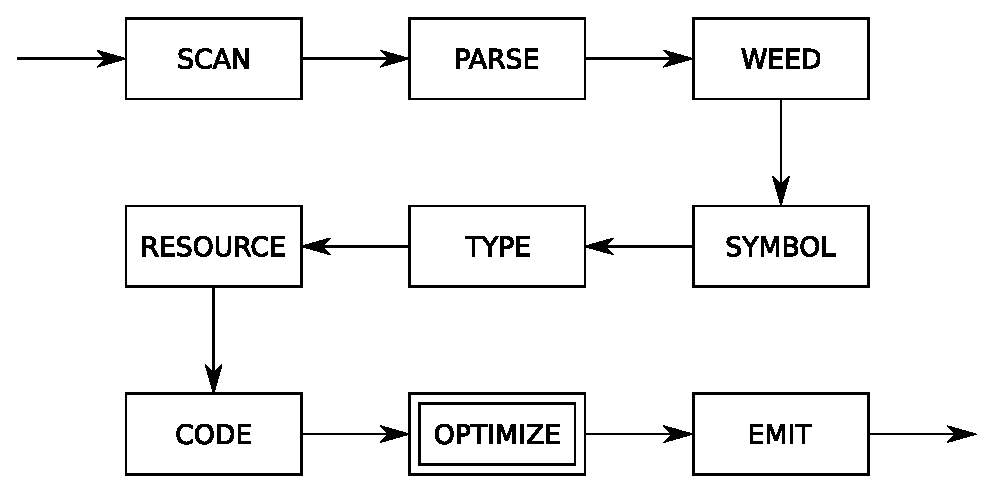
\psfig{file=figs/optimize.eps,width=20em}
\end{center}

\vfil
\end{slide*}
 
\begin{slide*}
The {\em optimizer\/} focuses on:
\begin{itemize}
\item reducing the execution time; or
\item reducing the code size; or 
\item reducing the power consumption (new).
\end{itemize}
These goals often conflict, since
a larger program may in fact be faster.

The best optimizations achieve both goals.
\vfil
\end{slide*}
 
\begin{slide*}
Optimizations for space:
\begin{itemize}
\item were historically very important, because memory was small and expensive;
\item when memory became large and cheap, optimizing compilers traded space for speed; but
\item then Internet bandwidth is small and expensive, so Java compilers optimize
for space, 
\item today Internet bandwidth is larger and cheaper, so we optimize for speed
again.
\end{itemize}
$\Rightarrow$ Optimizations driven by economy!

\vfil
\end{slide*}
 
\begin{slide*}
Optimizations for speed:
\begin{itemize}
\item were historically very important to gain acceptance for high-level languages;
\item are still important, since the software always strains the limits of the hardware;
\item are challenged by ever higher abstractions in programming languages; and
\item must constantly adapt to changing microprocessor architectures.
\end{itemize}
\vfil
\end{slide*}
 
\begin{slide*}
Optimizations may take place:
\begin{itemize}
\item at the source code level;
\item in an intermediate representation;
\item at the binary machine code level; or
\item at run-time (e.g.\ JIT compilers).
\end{itemize}
An aggressive optimization requires many small contributions from all levels.
\vfil
\end{slide*}

\begin{slide*}
Should you program in ``Optimized C''?\\

If you want a fast C program, 
should you use {\tt LOOP \#1} or {\tt LOOP \#2}? 

\begin{scriptsize}
\begin{verbatim}
/* LOOP #1 */
for (i = 0; i < N; i++) {
    a[i] = a[i] * 2000;
    a[i] = a[i] / 10000;
}

/* LOOP #2 */
b = a;
for (i = 0; i < N; i++) {
    *b = *b * 2000;
    *b = *b / 10000;
    b++;
}
\end{verbatim}
\end{scriptsize}
What would the expert programmer do?
\vfil
\end{slide*}

\begin{slide*}
If you said {\tt LOOP \#2} \ldots\ you were wrong!\\

\begin{center}
\begin{scriptsize}
\begin{tabular}{||l||c|c|c|c||}
\hline
{\tt LOOP} & opt. level & SPARC & MIPS & Alpha \\ \hline \hline
{\tt \#1} (array) & no opt &  20.5  & 21.6  & 7.85 \\ \hline
{\tt \#1} (array) & opt & 8.8  & 12.3  &  3.26\\ \hline
{\tt \#1} (array) & super &  7.9  & 11.2 & 2.96 \\ \hline \hline
{\tt \#2} (ptr)   & no opt & 19.5  & 17.6 & 7.55 \\ \hline
{\tt \#2} (ptr)   & opt & 12.4  & 15.4 & 4.09 \\ \hline
{\tt \#2} (ptr)   & super & 10.7  & 12.9 & 3.94 \\ \hline
\end{tabular}
\end{scriptsize}
\end{center}
\vspace*{2em}

\begin{itemize}
\item Pointers confuse most C compilers; don't use pointers instead of
array references.
\item Compilers do a good job of register allocation; don't try to
allocate registers in your C program.
\item In general, write clear C code; it is easier for both the programmer
and the compiler to understand.
\end{itemize}
\vfil
\end{slide*}
 
\begin{slide*}
Optimization in JOOS:
\begin{verbatim}
c = a*b+c;
if (c<a) a=a+b*113;
while (b>0) {
  a=a*c;
  b=b-1;
} 
\end{verbatim}
\vfil
\end{slide*}

\begin{slide*}
\renewcommand{\baselinestretch}{0.6}
\begin{center}
\vspace*{-.8cm}
\begin{scriptsize}
\begin{tabular}[t]{ccc}
\begin{minipage}{10em}
\begin{verbatim}
  iload_1
  iload_2
  imul
  iload_3
  iadd
  dup
  istore_3
  pop
  iload_3
  iload_1
  if_icmplt true_1
  iconst_0
  goto stop_2
  true_1:
  iconst_1
  stop_2:
  ifeq stop_0
  iload_1
  iload_2
  ldc 113
  imul
  iadd
  dup
  istore_1
  pop
  stop_0:
  start_3:
  iload_2
  iconst_0
  if_icmpgt true_5
  iconst_0
  goto stop_6
  true_5:
  iconst_1
  stop_6:
  ifeq stop_4
  iload_1
  iload_3
  imul
  dup
  istore_1
  pop
  iload_2
  iconst_1
  isub
  dup
  istore_2
  pop
  goto start_3
  stop_4:
\end{verbatim}
\end{minipage}
 &
\setlength{\unitlength}{0.00083300in}%
%
\begingroup\makeatletter\ifx\SetFigFont\undefined%
\gdef\SetFigFont#1#2#3#4#5{%
  \reset@font\fontsize{#1}{#2pt}%
  \fontfamily{#3}\fontseries{#4}\fontshape{#5}%
  \selectfont}%
\fi\endgroup%
\begin{picture}(624,24)(3289,-2773)
\thicklines
\put(3301,-2761){\vector( 1, 0){600}}
\end{picture}
 &
\begin{minipage}{10em}
\begin{verbatim}
  iload_1
  iload_2
  imul
  iload_3
  iadd
  istore_3
  iload_3
  iload_1
  if_icmpge stop_0
  iload_1
  iload_2
  ldc 113
  imul
  iadd
  istore_1
  stop_0:
  start_3:
  iload_2
  iconst_0
  if_icmple stop_4
  iload_1
  iload_3
  imul
  istore_1
  iinc 2 -1
  goto start_3
  stop_4:
\end{verbatim}
\end{minipage}
\end{tabular}
\end{scriptsize}
\end{center}
\renewcommand{\baselinestretch}{1}
\vfil
\end{slide*}
 
\begin{slide*}
Smaller and faster code:
\begin{itemize}
\item remove unnecessary operations;
\item simplify control structures; and
\item replace complex operations by simpler ones (strength reduction).
\end{itemize}
This is what the JOOS optimizer does.

Later, we shall look at:
\begin{itemize}
\item JIT compilers; and
\item more powerful optimizations based on static analysis.
\end{itemize}
\vfil
\end{slide*}
 
\begin{slide*}
Larger, but faster code: tabulation.

The sine function may be computed as:
$$
\mbox{\tt sin(}x\mbox{\tt )} = x - \frac{x^3}{3!} + \frac{x^5}{5!} - \frac{x^7}{7!} + \ldots...
$$
or looked up in a table:\\

\begin{scriptsize}
\begin{center}
\begin{tabular}{|l|l|}
\hline
{\tt sin(}0.0{\tt )} & 0.000000 \\\hline
{\tt sin(}0.1{\tt )} & 0.099833\\ \hline
{\tt sin(}0.2{\tt )} & 0.198669\\\hline
{\tt sin(}0.3{\tt )} & 0.295520\\\hline
{\tt sin(}0.4{\tt )} & 0.389418\\\hline
{\tt sin(}0.5{\tt )} & 0.479426\\\hline
{\tt sin(}0.6{\tt )} & 0.564642\\\hline
{\tt sin(}0.7{\tt )} & 0.644218\\\hline
& 
\end{tabular}
\end{center}
\end{scriptsize}
\vfil
\end{slide*}
 
\begin{slide*}
Larger, but faster code: loop unrolling.

The loop:

\begin{scriptsize}
\begin{verbatim}

for (i=0; i<2*N; i++) {
    a[i] = a[i] + b[i];
}

\end{verbatim}
\end{scriptsize}

is changed into:

\begin{scriptsize}
\begin{verbatim}

for (i=0; i<2*N; i=i+2) {
    j = i+1;
    a[i] = a[i] + b[i];
    a[j] = a[j] + b[j];
}

\end{verbatim}
\end{scriptsize}

which reduces the overhead and may give a 10--20\% speedup.

\vfil
\end{slide*}
 
\begin{slide*}
The optimizer must undo fancy language abstractions:
\begin{itemize}
\item variables abstract away from registers, so the optimizer must find an efficient mapping;
\item control structures abstract away from gotos, so the optimizer must construct and
simplify a goto graph;
\item data structures abstract away from memory, so the optimizer must find an efficient layout;
\item[$\vdots$]
\item method lookups abstract away from procedure calls, so the optimizer must efficiently
determine the intended implementations.
\end{itemize}
\vfil
\end{slide*}
 
\begin{slide*}
Continuing: the OO language BETA unifies as {\em patterns\/} the concepts:
\begin{itemize}
\item abstract class;
\item concrete class;
\item method; and
\item function.
\end{itemize}
A (hypothetical) optimizing BETA compiler must attempt to classify the 
patterns to recover that information.

Example: all patterns are allocated on the heap, but 50\% of the patterns are methods
that could be allocated on the stack.
\vfil
\end{slide*}

\begin{slide*}
Difficult compromises:
\begin{itemize}
\item a high abstraction level makes the development time cheaper, but the run-time
more expensive; however
\item high-level abstractions are also easier to analyze, which gives
optimization potential.
\end{itemize}
Also:
\begin{itemize}
\item an optimizing compiler makes run-time more efficient, but compile-time less
efficient;
\item optimizations for speed and size may conflict; and
\item different applications may require different optimizations.
\end{itemize}
\vfil
\end{slide*}
 
\begin{slide*}
The JOOS peephole optimizer:
\begin{itemize}
\item works at the bytecode level;
\item looks only at {\em peepholes}, which are sliding windows on the code sequence;
\item uses {\em patterns\/} to identify and replace inefficient constructions; 
\item continues until a global fixed point is reached; and
\item optimizes both speed and space.
\end{itemize}
\vfil
\end{slide*}
 
\begin{slide*}
The optimizer considers the goto graph:

\begin{scriptsize}
\begin{verbatim}
 while (a>0) {
   if (b==c) a=a-1; else c=c+1;
 }
\end{verbatim}
\end{scriptsize}

\vspace{2em}
\hspace*{4em}
\setlength{\unitlength}{0.0004700in}%
%
\begingroup\makeatletter\ifx\SetFigFont\undefined%
\gdef\SetFigFont#1#2#3#4#5{%
  \reset@font\fontsize{#1}{#2pt}%
  \fontfamily{#3}\fontseries{#4}\fontshape{#5}%
  \selectfont}%
\fi\endgroup%
\scalebox{.9}{
\begin{picture}(924,7530)(1189,-8347)
\thicklines
\put(2026,-1561){\line(-1, 0){225}}
\put(1801,-1561){\line( 0,-1){600}}
\put(1801,-2161){\vector( 1, 0){300}}
\put(2026,-2011){\line(-1, 0){300}}
\put(1726,-2011){\line( 0,-1){600}}
\put(1726,-2611){\vector( 1, 0){375}}
\put(2026,-3436){\line(-1, 0){225}}
\put(1801,-3436){\line( 0,-1){600}}
\put(1801,-4036){\vector( 1, 0){300}}
\put(2026,-3886){\line(-1, 0){300}}
\put(1726,-3886){\line( 0,-1){600}}
\put(1726,-4486){\vector( 1, 0){375}}
\put(2026,-4711){\line(-1, 0){225}}
\put(1801,-4711){\line( 0,-1){1650}}
\put(1801,-6361){\vector( 1, 0){300}}
\put(2026,-6211){\line(-1, 0){300}}
\put(1726,-6211){\line( 0,-1){1650}}
\put(1726,-7861){\vector( 1, 0){375}}
\put(2026,-2761){\line(-1, 0){525}}
\put(1501,-2761){\line( 0,-1){5475}}
\put(1501,-8236){\vector( 1, 0){600}}
\put(2026,-8086){\line(-1, 0){825}}
\put(1201,-8086){\line( 0, 1){7200}}
\put(1201,-886){\vector( 1, 0){900}}
\put(2101,-961){\makebox(0,0)[lb]{\smash{\SetFigFont{8}{14.4}{\ttdefault}{\mddefault}{\updefault}start\_0:}}}
\put(2101,-1171){\makebox(0,0)[lb]{\smash{\SetFigFont{8}{14.4}{\ttdefault}{\mddefault}{\updefault}iload\_1}}}
\put(2101,-1381){\makebox(0,0)[lb]{\smash{\SetFigFont{8}{14.4}{\ttdefault}{\mddefault}{\updefault}iconst\_0}}}
\put(2101,-1591){\makebox(0,0)[lb]{\smash{\SetFigFont{8}{14.4}{\ttdefault}{\mddefault}{\updefault}if\_icmpgt true\_2}}}
\put(2101,-1801){\makebox(0,0)[lb]{\smash{\SetFigFont{8}{14.4}{\ttdefault}{\mddefault}{\updefault}iconst\_0}}}
\put(2101,-2011){\makebox(0,0)[lb]{\smash{\SetFigFont{8}{14.4}{\ttdefault}{\mddefault}{\updefault}goto stop\_3}}}
\put(2101,-2221){\makebox(0,0)[lb]{\smash{\SetFigFont{8}{14.4}{\ttdefault}{\mddefault}{\updefault}true\_2:}}}
\put(2101,-2431){\makebox(0,0)[lb]{\smash{\SetFigFont{8}{14.4}{\ttdefault}{\mddefault}{\updefault}iconst\_1}}}
\put(2101,-2641){\makebox(0,0)[lb]{\smash{\SetFigFont{8}{14.4}{\ttdefault}{\mddefault}{\updefault}stop\_3:}}}
\put(2101,-2851){\makebox(0,0)[lb]{\smash{\SetFigFont{8}{14.4}{\ttdefault}{\mddefault}{\updefault}ifeq stop\_1}}}
\put(2101,-3061){\makebox(0,0)[lb]{\smash{\SetFigFont{8}{14.4}{\ttdefault}{\mddefault}{\updefault}iload\_2}}}
\put(2101,-3271){\makebox(0,0)[lb]{\smash{\SetFigFont{8}{14.4}{\ttdefault}{\mddefault}{\updefault}iload\_3}}}
\put(2101,-3481){\makebox(0,0)[lb]{\smash{\SetFigFont{8}{14.4}{\ttdefault}{\mddefault}{\updefault}if\_icmpeq true\_6}}}
\put(2101,-3691){\makebox(0,0)[lb]{\smash{\SetFigFont{8}{14.4}{\ttdefault}{\mddefault}{\updefault}iconst\_0}}}
\put(2101,-3901){\makebox(0,0)[lb]{\smash{\SetFigFont{8}{14.4}{\ttdefault}{\mddefault}{\updefault}goto stop\_7}}}
\put(2101,-4111){\makebox(0,0)[lb]{\smash{\SetFigFont{8}{14.4}{\ttdefault}{\mddefault}{\updefault}true\_6:}}}
\put(2101,-4321){\makebox(0,0)[lb]{\smash{\SetFigFont{8}{14.4}{\ttdefault}{\mddefault}{\updefault}iconst\_1}}}
\put(2101,-4531){\makebox(0,0)[lb]{\smash{\SetFigFont{8}{14.4}{\ttdefault}{\mddefault}{\updefault}stop\_7}}}
\put(2101,-4741){\makebox(0,0)[lb]{\smash{\SetFigFont{8}{14.4}{\ttdefault}{\mddefault}{\updefault}ifeq else\_4:}}}
\put(2101,-4951){\makebox(0,0)[lb]{\smash{\SetFigFont{8}{14.4}{\ttdefault}{\mddefault}{\updefault}iload\_1}}}
\put(2101,-5161){\makebox(0,0)[lb]{\smash{\SetFigFont{8}{14.4}{\ttdefault}{\mddefault}{\updefault}iconst\_1}}}
\put(2101,-5371){\makebox(0,0)[lb]{\smash{\SetFigFont{8}{14.4}{\ttdefault}{\mddefault}{\updefault}isub}}}
\put(2101,-5581){\makebox(0,0)[lb]{\smash{\SetFigFont{8}{14.4}{\ttdefault}{\mddefault}{\updefault}dup}}}
\put(2101,-5791){\makebox(0,0)[lb]{\smash{\SetFigFont{8}{14.4}{\ttdefault}{\mddefault}{\updefault}istore\_1}}}
\put(2101,-6001){\makebox(0,0)[lb]{\smash{\SetFigFont{8}{14.4}{\ttdefault}{\mddefault}{\updefault}pop}}}
\put(2101,-6211){\makebox(0,0)[lb]{\smash{\SetFigFont{8}{14.4}{\ttdefault}{\mddefault}{\updefault}goto stop\_5}}}
\put(2101,-6421){\makebox(0,0)[lb]{\smash{\SetFigFont{8}{14.4}{\ttdefault}{\mddefault}{\updefault}else\_4}}}
\put(2101,-6631){\makebox(0,0)[lb]{\smash{\SetFigFont{8}{14.4}{\ttdefault}{\mddefault}{\updefault}iload\_3}}}
\put(2101,-6841){\makebox(0,0)[lb]{\smash{\SetFigFont{8}{14.4}{\ttdefault}{\mddefault}{\updefault}iconst\_1}}}
\put(2101,-7051){\makebox(0,0)[lb]{\smash{\SetFigFont{8}{14.4}{\ttdefault}{\mddefault}{\updefault}iadd}}}
\put(2101,-7261){\makebox(0,0)[lb]{\smash{\SetFigFont{8}{14.4}{\ttdefault}{\mddefault}{\updefault}dup}}}
\put(2101,-7471){\makebox(0,0)[lb]{\smash{\SetFigFont{8}{14.4}{\ttdefault}{\mddefault}{\updefault}istore\_3}}}
\put(2101,-7681){\makebox(0,0)[lb]{\smash{\SetFigFont{8}{14.4}{\ttdefault}{\mddefault}{\updefault}pop}}}
\put(2101,-7891){\makebox(0,0)[lb]{\smash{\SetFigFont{8}{14.4}{\ttdefault}{\mddefault}{\updefault}stop\_5:}}}
\put(2101,-8101){\makebox(0,0)[lb]{\smash{\SetFigFont{8}{14.4}{\ttdefault}{\mddefault}{\updefault}goto start\_0}}}
\put(2101,-8311){\makebox(0,0)[lb]{\smash{\SetFigFont{8}{14.4}{\ttdefault}{\mddefault}{\updefault}stop\_1:}}}
\end{picture}
}

\vfil
\end{slide*}
 
\begin{slide*}
To capture the goto graph,
the labels for a given code sequence are represented as an array of:

\begin{small}
\begin{verbatim}
typedef struct LABEL {
   char *name;
   int sources;
   struct CODE *position;
} LABEL;
\end{verbatim}
\end{small}

where:

\begin{itemize}
\item the array index is the label's number;
\item the field {\tt name} is the textual part of the label;
\item the field {\tt sources} indicates the in-degree of the label; and
\item the field {\tt position} points to the location of the label in the code sequence.
\end{itemize}
\vfil
\end{slide*}
 
\begin{slide*}
Operations on the goto graph:
\begin{itemize}
\item inspect a given bytecode;
\item find the next bytecode in the sequence;
\item find the destination of a label;
\item create a new reference to a label;
\item drop a reference to a label;
\item ask if a label is dead (in-degree 0);
\item ask if a label is unique (in-degree 1); and
\item replace a sequence of bytecodes by another.
\end{itemize}
\vfil
\end{slide*}
 
\begin{slide*}
Inspect a given bytecode:

\begin{scriptsize}
\begin{verbatim}
int is_istore(CODE *c, int *arg)
{ if (c==NULL) return 0;
  if (c->kind == istoreCK) {
     (*arg) = c->val.istoreC;
     return 1;
  } else {
     return 0;
  }
}
\end{verbatim}
\end{scriptsize}

Find the next bytecode in the sequence:

\begin{scriptsize}
\begin{verbatim}
CODE *next(CODE *c)
{ if (c==NULL) return NULL;
  return c->next;
}
\end{verbatim}
\end{scriptsize}

Find the destination of a label:

\begin{scriptsize}
\begin{verbatim}
CODE *destination(int label)
{ return currentlabels[label].position;
}
\end{verbatim}
\end{scriptsize}

Create a new reference to a label:

\begin{scriptsize}
\begin{verbatim}
int copylabel(int label)
{ currentlabels[label].sources++;
  return label;
}
\end{verbatim}
\end{scriptsize}
\vfil
\end{slide*}

\begin{slide*}

Drop a reference to a label:

\begin{scriptsize}
\begin{verbatim}
void droplabel(int label)
{ currentlabels[label].sources--;
}
\end{verbatim}
\end{scriptsize}

Ask if a label is dead (in-degree 0):

\begin{scriptsize}
\begin{verbatim}
int deadlabel(int label)
{ return currentlabels[label].sources==0;
}
\end{verbatim}
\end{scriptsize}

Ask if a label is unique (in-degree 1):

\begin{scriptsize}
\begin{verbatim}
int uniquelabel(int label)
{ return currentlabels[label].sources==1;
}
\end{verbatim}
\end{scriptsize}

Replace a sequence of bytecodes by another:

\begin{scriptsize}
\begin{verbatim}
int replace(CODE **c, int k, CODE *r)
{ CODE *p;
  int i;
  p = *c;
  for (i=0; i<k; i++) p=p->next;
  if (r==NULL) {
     *c = p;
  } else {
     *c = r;
     while (r->next!=NULL) r=r->next;
     r->next = p;
  }
  return 1;
}
\end{verbatim}
\end{scriptsize}

\vfil
\end{slide*}
 
\begin{slide*}
The expression:

\begin{small}
\begin{verbatim}
x = x + k
\end{verbatim}
\end{small}

may be simplified to an increment operation, if 0~$\leq$~{\tt k}~$\leq$~127.\\

Corresponding JOOS peephole pattern:

\begin{scriptsize}
\begin{verbatim}

int positive_increment(CODE **c)
{ int x,y,k;
  if (is_iload(*c,&x) &&
      is_ldc_int(next(*c),&k) &&
      is_iadd(next(next(*c))) &&
      is_istore(next(next(next(*c))),&y) &&
      x==y && 0<=k && k<=127) {
     return replace(c,4,makeCODEiinc(x,k,NULL));
  }
  return 0;
}

\end{verbatim}
\end{scriptsize}

We may attempt to apply this pattern anywhere in the code sequence.
\vfil
\end{slide*}
 
\begin{slide*}
The algebraic rules:

\begin{small}
\begin{verbatim}
x * 0 = 0
x * 1 = x
x * 2 = x + x
\end{verbatim}
\end{small}

may be used to simplify some operations.\\

Corresponding JOOS peephole pattern:
 
\begin{scriptsize}
\begin{verbatim}
 
int simplify_multiplication_right(CODE **c)
{ int x,k;
  if (is_iload(*c,&x) && 
      is_ldc_int(next(*c),&k) && 
      is_imul(next(next(*c)))) {
     if (k==0) 
        return replace(c,3,makeCODEldc_int(0,NULL));
     else if (k==1) 
        return replace(c,3,makeCODEiload(x,NULL));
     else if (k==2) 
        return replace(c,3,makeCODEiload(x,
                           makeCODEdup(
                           makeCODEiadd(NULL))));
     return 0;
  }
  return 0;
}
\end{verbatim}
\end{scriptsize}
\vfil
\end{slide*}
 
\begin{slide*}
A part of the goto graph:

\hspace*{4em}
\setlength{\unitlength}{0.0004150in}%
%
\begingroup\makeatletter\ifx\SetFigFont\undefined%
\gdef\SetFigFont#1#2#3#4#5{%
  \reset@font\fontsize{#1}{#2pt}%
  \fontfamily{#3}\fontseries{#4}\fontshape{#5}%
  \selectfont}%
\fi\endgroup%
\begin{picture}(324,3480)(1789,-5197)
\thicklines
\put(2026,-1786){\line(-1, 0){225}}
\put(1801,-1786){\line( 0,-1){1500}}
\put(1801,-3286){\vector( 1, 0){300}}
\put(2101,-3511){\line(-1, 0){300}}
\put(1801,-3511){\line( 0,-1){1575}}
\put(1801,-5086){\vector( 1, 0){300}}
\put(2101,-1861){\makebox(0,0)[lb]{\smash{\SetFigFont{8}{14.4}{\ttdefault}{\mddefault}{\updefault}goto L\_1}}}
\put(2101,-3361){\makebox(0,0)[lb]{\smash{\SetFigFont{8}{14.4}{\ttdefault}{\mddefault}{\updefault}L\_1:}}}
\put(2101,-3571){\makebox(0,0)[lb]{\smash{\SetFigFont{8}{14.4}{\ttdefault}{\mddefault}{\updefault}goto L\_2}}}
\put(2101,-5161){\makebox(0,0)[lb]{\smash{\SetFigFont{8}{14.4}{\ttdefault}{\mddefault}{\updefault}L\_2:}}}
\end{picture}

may be simplified by short-circuiting the jump to {\tt L\_1}.\\

Corresponding JOOS peephole pattern:
 
\begin{scriptsize}
\begin{verbatim}

int simplify_goto_goto(CODE **c)
{ int l1,l2;
  if (is_goto(*c,&l1) && 
      is_goto(next(destination(l1)),&l2) && l1>l2) {
     droplabel(l1);
     copylabel(l2);
     return replace(c,1,makeCODEgoto(l2,NULL));
  }
  return 0;
}
\end{verbatim}
\end{scriptsize}
\vfil
\end{slide*}
 
\begin{slide*}
The JOOS peephole pattern:

\begin{scriptsize}
\begin{verbatim}
int simplify_astore(CODE **c)
{ int x;
  if (is_dup(*c) &&
      is_astore(next(*c),&x) &&
      is_pop(next(next(*c)))) {
     return replace(c,3,makeCODEastore(x,NULL));
  }
  return 0;
}
\end{verbatim}
\end{scriptsize}
is clearly sound, but will it ever be useful?\\

Yes, the assignment statement:

\begin{scriptsize}
\begin{verbatim}
a = b;
\end{verbatim}
\end{scriptsize}

generates the code:

\begin{scriptsize}
\begin{verbatim}
aload_2
dup
astore_1
pop
return
\end{verbatim}
\end{scriptsize}

because of our simpleminded strategy.

\vfil
\end{slide*}
 
\begin{slide*}
Coding assignments:

\begin{scriptsize}
\begin{verbatim}
void codeEXP(EXP *e) {
  case assignK:
    codeEXP(e->val.assignE.right);
    code_dup();
    ......
      case formalSym:
        if (e->val.assignE.leftsym->
               val.formalS->type->kind==refK) {
          code_astore(e->val.assignE.leftsym->
                         val.formalS->offset);
        } else {
          code_istore(e->val.assignE.leftsym->
                         val.formalS->offset);
        }
        break;
\end{verbatim}
\end{scriptsize}

To avoid the {\tt dup}, we must know if the assigned value is needed later;
this information must then flow back to the code:

\begin{scriptsize}
\begin{verbatim}
void codeSTATEMENT(STATEMENT *s) {
  case expK:
    codeEXP(s->val.expS);
    if (s->val.expS->type->kind!=voidK) {
       code_pop();
    }
    break;
\end{verbatim}
\end{scriptsize}

to decide whether to {\tt pop} or not. A peephole pattern is simpler and more modular.

\vfil
\end{slide*}
 
\begin{slide*}
Any collection of peephole patterns:

\begin{scriptsize}
\begin{verbatim}

typedef int(*OPTI)(CODE **);

#define MAX_PATTERNS 100

int init_patterns() {
  ADD_PATTERN(simplify_multiplication_right);
  ADD_PATTERN(simplify_astore);
  ADD_PATTERN(positive_increment);
  ADD_PATTERN(simplify_goto_goto);
  return 1;
}
\end{verbatim}
\end{scriptsize}

can be applied to a goto graph in a fixed point process:

\begin{small}
\begin{tabbing}
XX\=XX\=XX\=XX\=\kill
{\tt repeat}\\
\>{\tt for} each bytecode in succession {\tt do}\\
\>\>{\tt for} each peephole pattern in succession {\tt do}\\
\>\>\>{\tt repeat}\\
\>\>\>\>apply the peephole pattern\\
\>\>\>\>to the bytecode\\
\>\>\>{\tt until} the goto graph didn't change\\
\>\>{\tt end}\\
\>{\tt end}\\
{\tt until} the goto graph didn't change
\end{tabbing}
\end{small}
\vfil
\end{slide*}

\begin{slide*}

JOOS code for the fixed point driver:

\begin{scriptsize}
\begin{verbatim}

int optiCHANGE;
 
void optiCODEtraverse(CODE **c)
{ int i,change;
  change = 1;
  if (*c!=NULL) {
     while (change) {
       change = 0;
       for (i=0; i<OPTS; i++) {
           change = change | optimization[i](c);
       }
       optiCHANGE = optiCHANGE || change;
     }
     if (*c!=NULL) optiCODEtraverse(&((*c)->next));
  }
} 
 
void optiCODE(CODE **c)
{ optiCHANGE = 1;
  while (optiCHANGE) {
    optiCHANGE = 0;
    optiCODEtraverse(c);
  }
}
\end{verbatim}
\end{scriptsize}

\vfil
\end{slide*}
 
\begin{slide*}
Why does this process terminate?

Each peephole pattern does not necessarily make the code smaller.

To demonstrate termination for our examples, we use
the lexicographically ordered measure:

$$ <\mbox{\#bytecodes}, \mbox{\#{\tt imul}}, \sum_{\mbox{\tt L}} |\mbox{\em gotochain}(\mbox{\tt L})| >
$$

which can be seen to become strictly smaller after each application of a peephole pattern.
\vfil
\end{slide*}
 
\begin{slide*}
The goto graph obtained as a fixed point is {\em not\/} unique.

It depends on the sequence in which the peephole patterns are applied.

That does not happen for the four examples given, but consider the two peephole
patterns:\\

\begin{center}
\setlength{\unitlength}{0.00083300in}%
%
\begingroup\makeatletter\ifx\SetFigFont\undefined%
\gdef\SetFigFont#1#2#3#4#5{%
  \reset@font\fontsize{#1}{#2pt}%
  \fontfamily{#3}\fontseries{#4}\fontshape{#5}%
  \selectfont}%
\fi\endgroup%
\begin{picture}(2250,540)(1801,-2305)
\put(2551,-1936){\makebox(0,0)[lb]{\smash{\SetFigFont{12}{14.4}{\ttdefault}{\mddefault}{\updefault}A}}}
\put(2551,-2146){\makebox(0,0)[lb]{\smash{\SetFigFont{12}{14.4}{\ttdefault}{\mddefault}{\updefault}B}}}
\thicklines
\put(1951,-2011){\vector( 1, 0){525}}
\put(3451,-2011){\vector( 1, 0){525}}
\put(1801,-1861){\makebox(0,0)[lb]{\smash{\SetFigFont{12}{14.4}{\ttdefault}{\mddefault}{\updefault}A}}}
\put(1801,-2071){\makebox(0,0)[lb]{\smash{\SetFigFont{12}{14.4}{\ttdefault}{\mddefault}{\updefault}B}}}
\put(1801,-2281){\makebox(0,0)[lb]{\smash{\SetFigFont{12}{14.4}{\ttdefault}{\mddefault}{\updefault}C}}}
\put(2101,-1936){\makebox(0,0)[lb]{\smash{\SetFigFont{12}{14.4}{\ttdefault}{\mddefault}{\updefault}$P_1$}}}
\put(3301,-1936){\makebox(0,0)[lb]{\smash{\SetFigFont{12}{14.4}{\ttdefault}{\mddefault}{\updefault}C}}}
\put(3301,-2146){\makebox(0,0)[lb]{\smash{\SetFigFont{12}{14.4}{\ttdefault}{\mddefault}{\updefault}D}}}
\put(4051,-1936){\makebox(0,0)[lb]{\smash{\SetFigFont{12}{14.4}{\ttdefault}{\mddefault}{\updefault}D}}}
\put(4051,-2146){\makebox(0,0)[lb]{\smash{\SetFigFont{12}{14.4}{\ttdefault}{\mddefault}{\updefault}E}}}
\put(3601,-1936){\makebox(0,0)[lb]{\smash{\SetFigFont{12}{14.4}{\ttdefault}{\mddefault}{\updefault}$P_2$}}}
\end{picture}
\end{center}

They clearly do not commute:

\begin{center}
\setlength{\unitlength}{0.00083300in}%
%
\begingroup\makeatletter\ifx\SetFigFont\undefined%
\gdef\SetFigFont#1#2#3#4#5{%
  \reset@font\fontsize{#1}{#2pt}%
  \fontfamily{#3}\fontseries{#4}\fontshape{#5}%
  \selectfont}%
\fi\endgroup%
\begin{picture}(1812,1800)(1801,-4915)
\put(2701,-4261){\makebox(0,0)[lb]{\smash{\SetFigFont{12}{14.4}{\ttdefault}{\mddefault}{\updefault}A}}}
\put(2701,-4471){\makebox(0,0)[lb]{\smash{\SetFigFont{12}{14.4}{\ttdefault}{\mddefault}{\updefault}B}}}
\put(2701,-4681){\makebox(0,0)[lb]{\smash{\SetFigFont{12}{14.4}{\ttdefault}{\mddefault}{\updefault}D}}}
\put(2701,-4891){\makebox(0,0)[lb]{\smash{\SetFigFont{12}{14.4}{\ttdefault}{\mddefault}{\updefault}E}}}
\put(3601,-4261){\makebox(0,0)[lb]{\smash{\SetFigFont{12}{14.4}{\ttdefault}{\mddefault}{\updefault}A}}}
\put(3601,-4471){\makebox(0,0)[lb]{\smash{\SetFigFont{12}{14.4}{\ttdefault}{\mddefault}{\updefault}B}}}
\put(3601,-4681){\makebox(0,0)[lb]{\smash{\SetFigFont{12}{14.4}{\ttdefault}{\mddefault}{\updefault}D}}}
\put(3601,-4891){\makebox(0,0)[lb]{\smash{\SetFigFont{12}{14.4}{\ttdefault}{\mddefault}{\updefault}E}}}
\thicklines
\put(1951,-3811){\vector( 3, 2){675}}
\put(2851,-3361){\vector( 1, 0){720}}
\put(1951,-4036){\vector( 3,-2){675}}
\put(2851,-4486){\vector( 1, 0){720}}
\put(1801,-3661){\makebox(0,0)[lb]{\smash{\SetFigFont{12}{14.4}{\ttdefault}{\mddefault}{\updefault}A}}}
\put(1801,-3871){\makebox(0,0)[lb]{\smash{\SetFigFont{12}{14.4}{\ttdefault}{\mddefault}{\updefault}B}}}
\put(1801,-4081){\makebox(0,0)[lb]{\smash{\SetFigFont{12}{14.4}{\ttdefault}{\mddefault}{\updefault}C}}}
\put(1801,-4291){\makebox(0,0)[lb]{\smash{\SetFigFont{12}{14.4}{\ttdefault}{\mddefault}{\updefault}D}}}
\put(2701,-3211){\makebox(0,0)[lb]{\smash{\SetFigFont{12}{14.4}{\ttdefault}{\mddefault}{\updefault}A}}}
\put(2701,-3421){\makebox(0,0)[lb]{\smash{\SetFigFont{12}{14.4}{\ttdefault}{\mddefault}{\updefault}B}}}
\put(2701,-3631){\makebox(0,0)[lb]{\smash{\SetFigFont{12}{14.4}{\ttdefault}{\mddefault}{\updefault}D}}}
\put(3601,-3211){\makebox(0,0)[lb]{\smash{\SetFigFont{12}{14.4}{\ttdefault}{\mddefault}{\updefault}A}}}
\put(3601,-3421){\makebox(0,0)[lb]{\smash{\SetFigFont{12}{14.4}{\ttdefault}{\mddefault}{\updefault}B}}}
\put(3601,-3631){\makebox(0,0)[lb]{\smash{\SetFigFont{12}{14.4}{\ttdefault}{\mddefault}{\updefault}D}}}
\put(2101,-3461){\makebox(0,0)[lb]{\smash{\SetFigFont{12}{14.4}{\ttdefault}{\mddefault}{\updefault}$P_1^*$}}}
\put(2101,-4486){\makebox(0,0)[lb]{\smash{\SetFigFont{12}{14.4}{\ttdefault}{\mddefault}{\updefault}$P_2^*$}}}
\put(3076,-3236){\makebox(0,0)[lb]{\smash{\SetFigFont{12}{14.4}{\ttdefault}{\mddefault}{\updefault}$P_2^*$}}}
\put(3076,-4361){\makebox(0,0)[lb]{\smash{\SetFigFont{12}{14.4}{\ttdefault}{\mddefault}{\updefault}$P_1^*$}}}
\end{picture}
\end{center}
\vfil
\end{slide*}
 
\begin{slide*}
The effect of the JOOS A+ optimizer\\(using 40 peephole patterns):\\

{\tt
\begin{scriptsize}
\begin{center}
\begin{tabular}{|l|r|r|}
\hline
{\rm Program} & joosa+ & joosa+ -O\\\hline\hline
AllComponents & 907 & 861\\\hline
AllEvents & 1056 & 683\\\hline
Animator & 184 & 180\\\hline
Animator2 & 568 & 456\\\hline
ConsumeInteger & 164 & 107\\\hline
DemoFont & 97 & 89\\\hline
DemoFont2 & 213 & 147\\\hline
DrawArcs & 60 & 60\\\hline
DrawPoly & 94 &  90\\\hline
Imagemap & 470 & 361\\\hline
MultiLineLabel & 526 & 406\\\hline
ProduceInteger & 149 & 96\\\hline
Rectangle2 & 58 & 58\\\hline
ScrollableScribble & 566 & 481\\\hline
ShowColors & 88 & 68\\\hline
TicTacToe & 1471 & 1211\\\hline
YesNoDialog & 315 & 248\\\hline
\end{tabular}
\end{center}
\end{scriptsize}
}

\vfil
\end{slide*}
 
\begin{slide*}
The word ``optimizer'' is somewhat misleading, since the code is not optimal but
merely better.

Suppose $\mbox{\em OPM}(G)$ is the shortest goto graph equivalent to $G$.

Clearly, the shortest diverging goto graph is:

\begin{center}
$D_{\mbox{min}}$ ~~=~~~ \begin{minipage}{4em}
\begin{verbatim}
L:
goto L
\end{verbatim}
\end{minipage}
\end{center}

We can then decide the Halting problem on an arbitrary goto graph $G$ as:
$$ \mbox{\em OPM}(G) = D_{\mbox{min}} $$
Hence, the program {\em OPM\/} cannot exist.
\vfil
\end{slide*}
 
\begin{slide*}
The testing strategy for the optimizer has three phases.\\

First a careful argumentation that each peephole pattern is sound.\\

Second a demonstration that each peephole pattern is realized correctly.\\

Third a statistical analysis showing that the optimizer improves the generated
programs.
\vfil
\end{slide*}
 
\begin{slide*}
\vfil
\end{slide*}
 
\begin{slide*}
\vfil
\end{slide*}
 
\begin{slide*}
\vfil
\end{slide*}
 
\begin{slide*}
\vfil
\end{slide*}
 
\begin{slide*}
\vfil
\end{slide*}
 
\end{document}

